\flchap{Location Prediction}

Based on the questions we answered in the previous section, we have enough
information to build a system for location prediction, which we call
FriendlyLocation.
%
Since the location prediction system will be run on a large number of users,
it must be fast and scalable.
%
In Chapter~\ref{chap:eval} we will evaluate this system using five-fold cross
validation.
%
In this chapter we will use the numbers from one of the five folds to make
the descriptions more concrete.


\flsec{Baseline: The Facebook Model}
The Facebook model developed by Backstrom et al. \cite{backstrom2010find}
begins with a striking observation: that the probability of friendship is
roughly inversely proportional to distance.
%
Specifically, by examining the ratio of actual edges at a particular distance
to the total number of possible edges at that distance (i.e., the probability
of friendship), they find a curve of the form $a(b+x)^{-c}$, with an exponent
close to $c=-1$.

\begin{figure}[tbh]
\centering
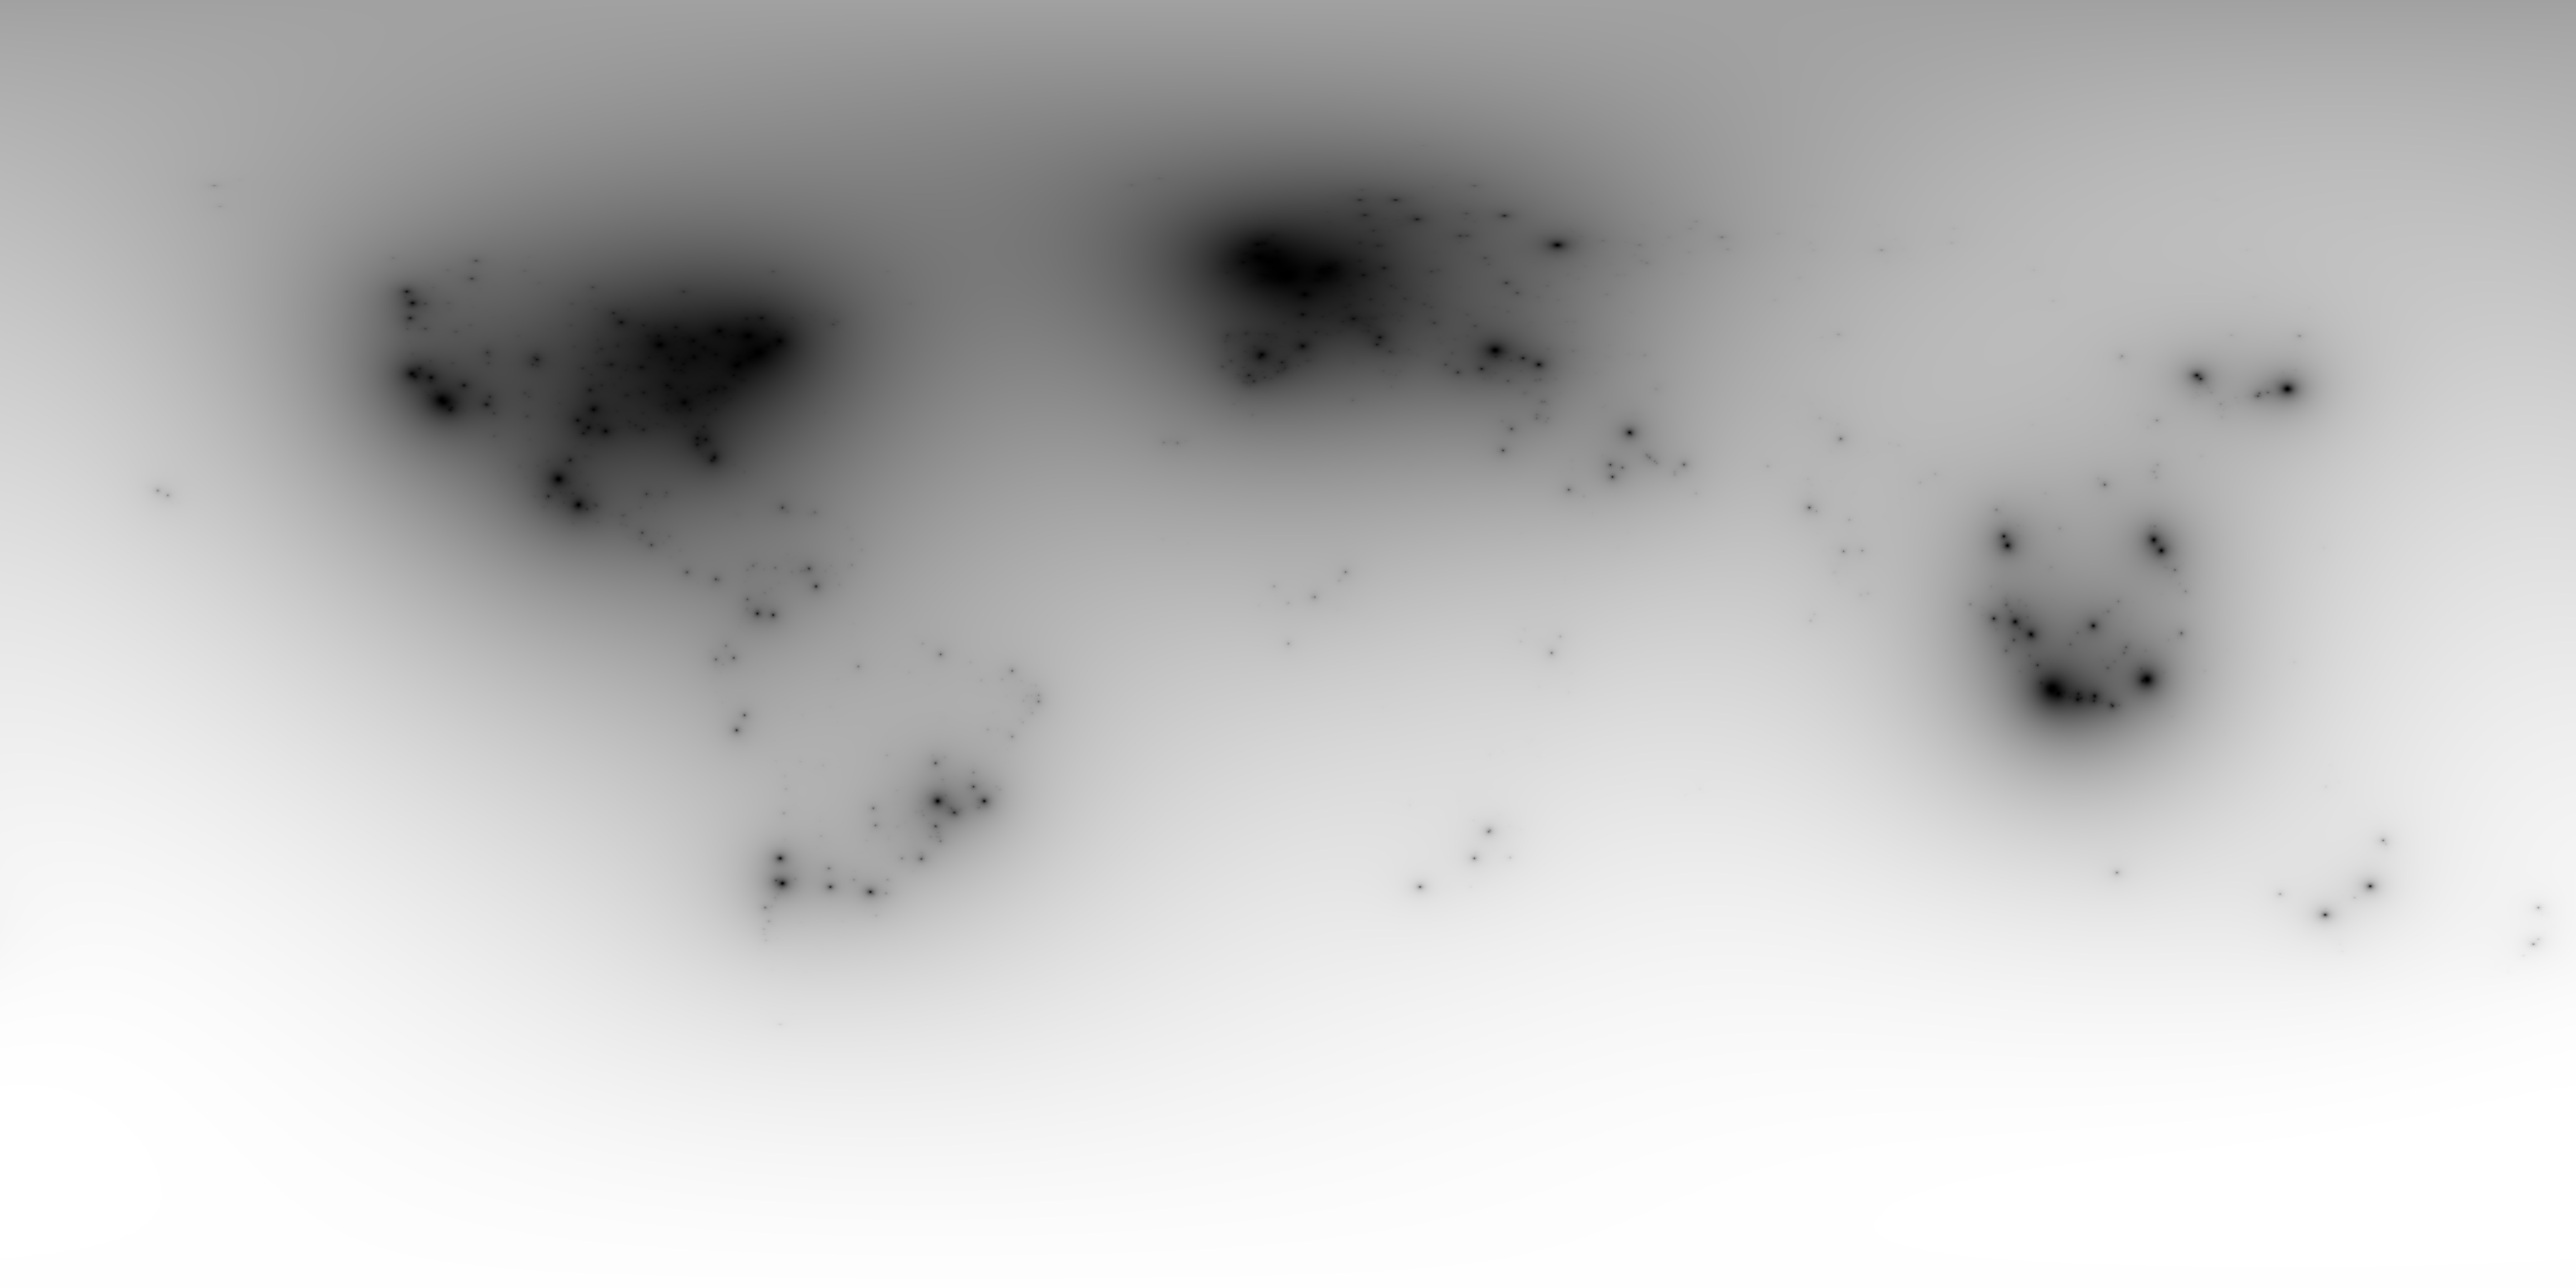
\includegraphics[width=\linewidth]{figures/stranger_mat.png}
\caption{
    This is the probability that a user lives at a location based on the people
    who they have no contact with. Dark areas have lower probability, and light
    areas have a higher probability.
}
\label{fig:StrangerMat}
\end{figure}

With the empirically observed probability of friendship, they can estimate the
likelihood that a user lives at a location $l$ using both $L^c$, the set of
locations of the user's friends with known locations, and $L^s$, all 2.9
million known locations of Facebook users.
%
Then, the Facebook model estimates the likelihood of location $l$ as:
\[
    \Backstrom(l,L^c) =
        \prod_{l^c \in L^c} {\p(|l-l^c|) \over 1-\p(|l-l^c|) }
        \prod_{l^s \in L^s} 1-\p(|l-l^s|)
\]

\noindent where $\p$ is the probability of friendship given an input distance
(which again, can be derived empirically).
%
The first product in the formula combines the probabilities from a user's friends.
%
Locations near a user's friends will have a higher probability because $\p$ is
roughly inversely proportional to distance.
%
The last product in the likelihood formula is only a function of the location
$l^c_i$ and the locations of the strangers; it does not depend on any other
information about the target user's contacts.
%
For convenience, we refer to this as $\pStrangers$:
\[
    \pStrangers(l) = \prod_{l^s \in L^s}1-p(|l-l^s|)
\]

\noindent As suggested in \cite{backstrom2010find}, this can be pre-computed
for every location.
%
Figure~\ref{fig:StrangerMat} shows $\pStrangers$ for every location on earth.
%
Major cities have the lowest probability for
$\pStrangers$, and remote areas have the highest probability.  It may seem
counter-intuitive that areas with low population density have a higher
probability, but consider this example: if someone has ten friends in New York
City and ten friends in a small town in upstate New York, they are more likely
to live in the small town, and just happen to know people in the big city.

The Facebook model naturally aggregates the locations of a user's friends, and
gives the probability that a user lives at a given location.
%
They then calculate this probability at each of the locations of the user's friends.
%
The location with the highest probability is often the center of the cluster of
the user's friends.
%
However, directly applying this approach to other non-Facebook domains may
encounter difficulties.
%
First, the Facebook empirical study focused only on the continental US, meaning
that distances between contacts were naturally limited to around 1,000 miles.
%
When investigating global friendships (as on Twitter or on the rest of
Facebook), there is considerable noise introduced in the 1,000--10,000 mile
range due to the distribution of land and oceans on the surface of the earth.
%
Second, the Facebook dataset had street addresses for approximately 2.9 million
Americans, and they used the friendships between users with street addresses to
do the calculation.
%
Since information on Facebook is usually only shared with a user's friends,
people are more willing to divulge their home addresses.
%
On most other social media websites, the location is publicly shared.
%
In practice, many users in social media reveal broad, imprecise
locations (e.g., at the city or state level), while others provide fine-grained
latitude-longitude information.
%
Third, the strength of connection between users necessarily varies, so
capturing this variation is important.
%
Encouragingly, Gilbert \cite{gilbert2009predicting} have shown how the strength
of a tie can be predicted by interaction patterns.
%
Finally, many social systems serve different purposes.
%
Twitter, for example, is both a social network connecting friends (which may
tend to be local) as well as a news media (supporting global dissemination)
\cite{kwak2010why}.


\flsec{Edge Length Classification}

A common theme of these challenges is that the quality of the geographic
information conveyed by a relationship in social media varies.
%
Some edges may convey strong evidence of the location of a user.
%
For example, intuitively the many edges between a user with an unknown location
and his co-workers (for whom we know their location) should contribute strongly
to the likelihood that the user is nearby those co-workers.
%
In contrast, links between a user with an unknown location and with a news
service (e.g., CNN) should contribute little discriminating power to estimating
the location of the user.

The challenge here is to separate the best contacts, who are likely to be
nearby, from bad contacts who are likely to be far away.
%
The factors that we investigated in the previous section indicate when someone
is likely to be nearby, but they don't guarantee it.
%
There are pairs of users who are reciprocal friends with a small number of
followers, a high local friend ratio, have conversations, and still live on
opposite sides of the globe.
%
Another problem with this data is that some of these factors are correlated
with each other; users with lots of followers tend to have a low friend contact
ratio.
%
Finally, distant accounts like celebrities may be useless for determining which
city a person is from, but they might still suggest the user's home country.

In \cite{backstrom2010find}, the authors present a model of the relationship
between distance and friendship that treats all of the edges the same.
%
We can improve the accuracy of this model by weighting some edges more strongly
than others.
%
We have several pieces of information, and want to map it to a single, extremely
noisy value: the distance to a contact.
%
This could be looked at as a classification problem where you want to classify
edges as local or non-local, but the problem is there is a smooth continuum
from local to non-local, and semi-local friends can be useful for location
prediction.
%
As a result, we model this as a regression problem.
%
Since most of the input features are correlated and either binary or non-linear,
linear regression is unlikely to work well.
%
In addition, the data is dense and low-dimensional, so Support Vector Machines
do not work well.
%
We chose to use a decision tree regressor based on the CART algorithm
(classification and regression trees) to distinguish the best edges from the
worst.
%
A decision tree regressor works similar to the well-known decision tree
classifier, except that it produces real numbers as output instead of discrete
classes.
%
During training, the training data is recursively split based on the input
variable with the most predictive power to build a binary tree.
%
Each of the internal nodes of this tree have a cutoff for one of the input
variables, and the leaves of the tree have a predicted value.

The regression tree was trained on several of the features from the previous
section that are correlated with users living near each other:
\begin{itemize}
\item the type of contact
\item if the target mentioned the contact
\item if the contact mentioned the target
\item if the contact had a protected account
\item the contact's follower and friend count
\item the MLE of the contact's location
\item the contact's local friend ratio
\end{itemize}
%
Since the distances between users varied by several orders of magnitude, we
trained the regressor to predict the log of the distance.
%
The tree regressor was configured to not split leafs with fewer than 1000 data
points to prevent over-fitting.
%
The top three levels of a decision tree are shown in Figure~\ref{fig:TreeTop}.
%
The predictor does not do a great job of predicting the actual distance to a
contact; there's simply too much noise.
%
However, it does do an excellent job of separating the closest pairs of users
from the most distant pairs as we will show in the next section.

\begin{figure}[tbh]
\centering
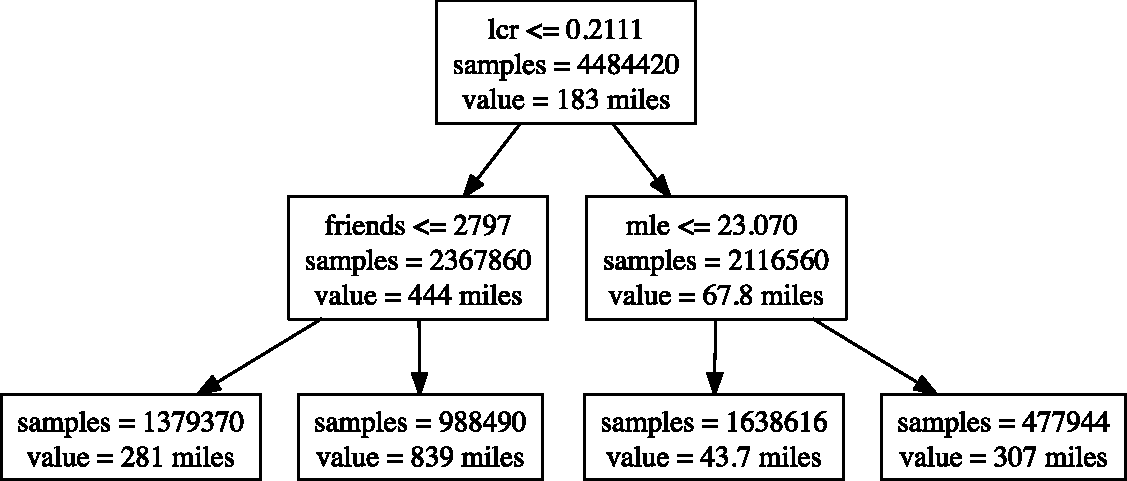
\includegraphics[width=\linewidth]{figures/tree_top.pdf}
\caption{
    The top three levels of the decision tree. This decision tree will predict a
    distance of 839 miles for a contact with a local contact ratio of .2 and
    2800 friends. It will predict a much-closer distance of 43.7 miles for a
    user with a local contact ratio of .5 and a predicted location error of 10
    miles.
}
\label{fig:TreeTop}
\end{figure}

\flsec{FriendlyLocation Prediction System}
\label{sec:model}

In the previous sections, we looked at the probability that a contact lives a
certain distance from a given user.
%
In this section, we build a model for the probability that a user, who we refer
to as the target user, lives at a specific location given the approximate
location of his contacts.
%
We use this to extend the baseline maximum likelihood estimator.


Just like \cite{backstrom2010find}, we can find that probability by comparing
the distribution of Twitter users to the distribution of the contacts.
%
First, we need a model for the density of Twitter users.
%
We calculate the distance between every target user and every contact
(even for contacts and users who had no relationship).
%
We call the number of target and contact pairs that are $d$ miles apart
$\edges(d)$.

Next, we need to model the probability that two users are contacts.
%
We propose to assess the relative quality of each edge from a target
user to his contacts, so that edges conveying strong location information are
weighed more than others.
%
Concretely, suppose we have a single edge from a user to one of his contacts.
%
We propose to assign this edge to a quantile based on its estimated
``goodness'' as determined by the decision tree.
%
We will show that the tree regressor described in the previous section does a
reasonable job of sorting out good and bad edges.

This decision tree will give us a set of $n$ predicted lengths $d^p_i \in D^p$
that correspond to the $n$ actual lengths of the edges $d^a_i \in D^a$.
%
Suppose we construct a set of $m$ quantiles, representing edges at different
predicted distances.
%
Let the boundaries for these quantiles be $\{q_0,\dots,q_m\}$,
where:\footnote{The notation used for order statistic may need some
    explanation.  $X_{(n)}$ is the $n^{th}$ element in the set $X$ when sorted
    in increasing order, so $X_{(2)}$ means the second smallest element in
$X$.}
\[
    q_j =
    \begin{cases}
        D^p_{(1+\lfloor {jn\over m} \rfloor)}, & j<m \\
        \infty & j=m
    \end{cases}
\]
\noindent The quantile for a specific distance $d^p_i$ can be found by
comparing it to the boundaries:
\[
    \quantile(d^p_i) = \max_{j \in \{0,\dots,m\}} \{j: d^p_i<q_j\}
\]

Hence, we can identify the actual edges ($\actEdges$) that exist with a distance of $d$.
%
This lets us find $\actEdges$, which is the number of users who fit in a quantile $j$ and had an actual distance of $d$
\[
    \actEdges(j,d) = |\{
            i \in \{1,\dots,n\} :
            d=d^a_i \wedge j=\quantile(d^p_i)
        \}|
\]

By comparing the number of edges that could have existed to the number of edges
that actually exist at a specific distance and in a specific quantile, we can
find the probability that a contact at a specific distance is in a quantile:

\[
\pContact(j,d) = \frac{\actEdges(j,d)}{\edges(d)}
\]

\begin{figure}[tbh]
\centering
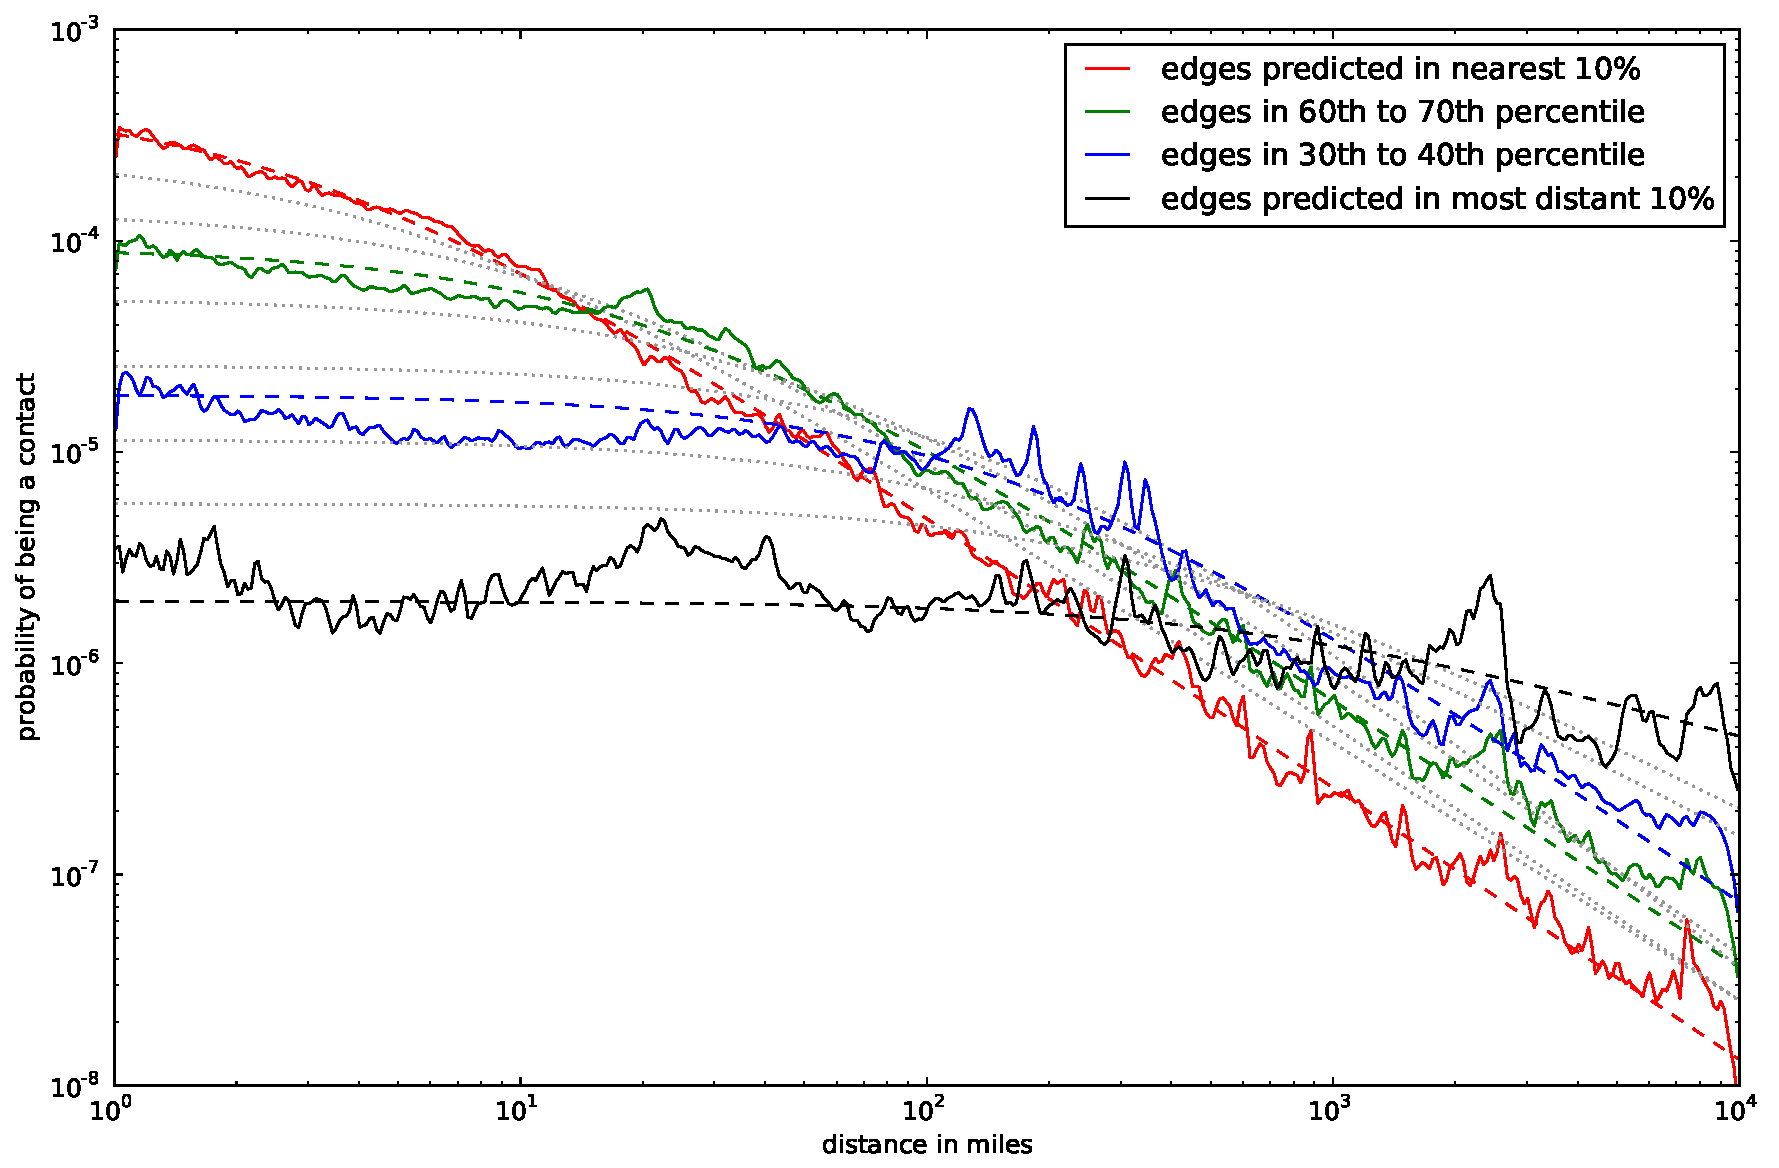
\includegraphics[width=\linewidth]{figures/vect_fit.pdf}
\caption{
After splitting edges into groups based on their predicted distance, each group
was fit to a curve. Here are four of the ten curves and their curves of best
fit. The other six curves of best fit are shown as faint dotted lines. The
decision tree does a reasonable job of separating the best edges from the worst
edges.
}
\label{fig:NearProbFit}
\end{figure}

We choose to split into ten quantiles, which gave us ten different curves for the
probability that a certain type of contact exists between a pair of users.
%
Four of the ten curves from one of the folds from the five-fold evaluation and
their lines of best fit are shown in Figure~\ref{fig:NearProbFit}.
%
The best contacts are orders of magnitude more
likely to live near a target user than the worst contacts.
%
If the predictions from the tree regressor were ignored, and users were placed
into one group instead of ten equal groups, this would reduce to the model
for friendship and distance presented in \cite{backstrom2010find}.
%
We choose ten because it was large enough to distinguish between the curves.
%
Larger numbers of quantiles give no benefit since the curves we are
fitting are so noisy as can be seen in Figure~\ref{fig:NearProbFit}.


We can combine this improved model into the existing estimator by
replacing the probability of being a contact based purely on distance ($p$) to
the probability based on the regression tree ($\pContact$).
%
We now have a formula for predicting the best location given $L$, the set of
locations of the contacts, and $P$, the set of predicted distances to the same
contacts:
\[
    FL(l,L,P) =
        \left(
            \prod_{l^c_k \in L,p_k \in P}
            {\pContact(\quantile(p_k),|l-l^c_k|) \over (1-p(|l-l^c_k|))}
        \right)
        \pStrangers(l)
\]


Algorithm~\ref{alg:friendloc} shows all the pieces from this section and the
previous section tied together.

\begin{algorithm}
  %\label{alg:friendloc}
  \caption{FriendlyLocation \label{alg:friendloc}}
  \begin{algorithmic}[0]
  \Input{The contacts $contacts$}
  \Output{The predicted location}
  \State locations = list()
  \State predictedDists = list()
  \ForEach{contact \textbf{in} contacts}
      \If{contact.location \textbf{is} None}
        \State \Continue
      \EndIf
      \State locations.append(contact.location)
      \State dist = regressionTree.predict(contact.features)
      \State predictedDists.append(dist)
  \EndFor
  \State best = argmax(FriendLoc(locations,predictedDists))
  \State \Return locations[best]
  \end{algorithmic}
\end{algorithm}

%\jam{locations of contacts are not independent as seen in~\ref{sec:closer}, but
%this formula really assumes they are. Where do we want to talk about this?}

